% Latex Template
%
% Fall 2015
%
% Created by: Andy Sayler
% Modified by: Taylor Andrews

\documentclass[11pt,twocolumn,letterpaper]{article}

% System Packages
\usepackage{epsfig}
\usepackage{float}
\usepackage{caption}
\usepackage{subcaption}
\usepackage{tabu}
\usepackage{color}
\usepackage{hyperref}
\usepackage{url}

% Local Packages
% None

% Package Options
\hypersetup{
    colorlinks,
    citecolor=black,
    filecolor=black,
    linkcolor=black,
    urlcolor=black
}

% Macros
\newenvironment{packed_enum}{
\begin{enumerate}
  \setlength{\itemsep}{1pt}
  \setlength{\parskip}{0pt}
  \setlength{\parsep}{0pt}
}{\end{enumerate}}

\newenvironment{packed_item}{
\begin{itemize}
  \setlength{\itemsep}{1pt}
  \setlength{\parskip}{0pt}
  \setlength{\parsep}{0pt}
}{\end{itemize}}

\newenvironment{packed_desc}{
\begin{description}
  \setlength{\itemsep}{1pt}
  \setlength{\parskip}{0pt}
  \setlength{\parsep}{0pt}
}{\end{description}}


% Other Options
\clubpenalty = 10000
\widowpenalty = 10000

% Variables
\newcommand{\appname}{FuseBox }
\newcommand{\appnameWOspace}{FuseBox}

\newcommand{\custos}{Tutamen }
\newcommand{\custosWOspace}{Tutamen}

% Start
\begin{document}

\title{\appname}

\author{Taylor Andrews}

\maketitle

\begin{abstract}
Security in the digital age is an ever evolving problem.
Services are doing their very best to protect sensitive data. 
However, in the face of social engineering attacks and other more technical
exploits, it can be on the user to go the extra step to make sure
their data is safe. Safety, however, should not come at the cost of
sharing data between trusted people and devices. Take Dropbox for
example \cite{exampleref1}. It supports many sharing features, so users can't just
encrypt and decrypt their files on a single computer. A more robust,
and shareable, way to encrypt files is needed. 
\appname aims to be a solution to this problem by providing a
transparent layer of security between the end user and Dropbox. Files
that pass through \appname are encrypted when uploaded to Dropbox. 
Encryption, decryption, and authentication are all supported by \appnameWOspace.
%Shareability is provided using Custos, a ``Secret Storage as a Service''
%(SSaaS) platform CITATION?. Custos allows for key sharing amongst
%people and computers. 
This paper will lay out
the design and implementation of \appnameWOspace, as well as 
future goals for the project.    
\end{abstract}

\section{Introduction}
\label{sec:intro}
Unsecured data is a gamble, a risk. No one wants to think that
they could be the target of an attack. The idea of keeping things safe
is nothing complicated. However, to the layman, the intricacies of
actually protecting data are somewhat out of reach. This problem
becomes compounded when a single person wants to safely share data
with trusted partners. Cloud-based products, like Dropbox, are built
on the ability to share and transfer data. How can users protect their
data while still being able to normally use Dropbox? 
\par Fortunately, part of the solution to this problem already exits.
\custosWOspace, a ``Secret Storage as a Service'' (SSaaS), 
provides a flexible means of storing and
retrieving secrets \cite{exampleref1}. The SSaaS model supports the features of
Dropbox that \appname needs to interact with. Leveraging \custos allows \appname to 
authenticate in conjunction with cloud based services. The user's
identity can be confirmed, and the appropriate key retrieved, on any number
of platforms. In addition, \custos provides the user with the 
flexibility to choose how they want to authenticate themselves. 
\par Getting a key in this manner relieves the problems associated
with using the cloud. The user's data, however, still needs to be
protected. \appname aims to accomplish this as transparently as
possible. To the end user, it appears that they are just normally
interacting with their Dropbox. They can read, write, and create
files. These files, from the perspective of Dropbox, are actually
encrypted. If Dropbox is somehow compromised, data that passes through \appname
will not be.    

\subsection{Goals}
\label{sec:goals}
\appname was created with two primary goals: transparency and consistency. 
\par {\bf Transparency:} Dropbox is a very convenient application to
use. Put files in, get files out. The existing desktop application
allows for seamlessly uploading and downloading files \cite{exampleref1}. The end user
gets to take advantage of all the nice features of Dropbox at little
to no effort on their end. \appname is built to keep this same 
seamless feel while preserving the features of Dropbox. Meanwhile behind the
scenes encryption, decryption, and authentication work together to
secure the data.     
\par {\bf Consistency:} \appnameWOspace's performance is bound by
the speed of internet because it must connect to Dropbox. 
\appname does not seek to overcome this
limitation. Rather, regardless of file type or file size, the client
is designed to perform equally well. Larger files should not create
massive latency when using \appnameWOspace. This means the user is not
limited when using the client.    

\section{Design}
\label{sec:design}
\appname is, in essence, an encrypted file system built on
Dropbox. Its main components are as follows:
\par {\bf File System:} 
\par {\bf Encryption:} 
\par {\bf Key Storage:}  

\subsection{File System}
\label{sec:fs}
FUSE  Dropbox API

\subsection{Encryption}
\label{sec:enc}
AES stream cipher

\subsection{Key Storage}
\label{sec:keystorage}
this is \custos

\section{Implementation}
\label{sec:implementation}

How did I accomplish the design?

\section{Conclusion}
\label{sec:conclusion}

Where do we go from here?

\section{Examples}
\label{sec:ex}

\noindent
This is a citation~\cite{exampleref1}.

% The tilde (~) in the previous sentence is optional, and just helps
% to insure citations and references don't wind up on a new line
% separated from the text they're attached to.

% noindent can be used to prevent indentation on single-line paragraphs.

\begin{figure}[htb]
  \centering
  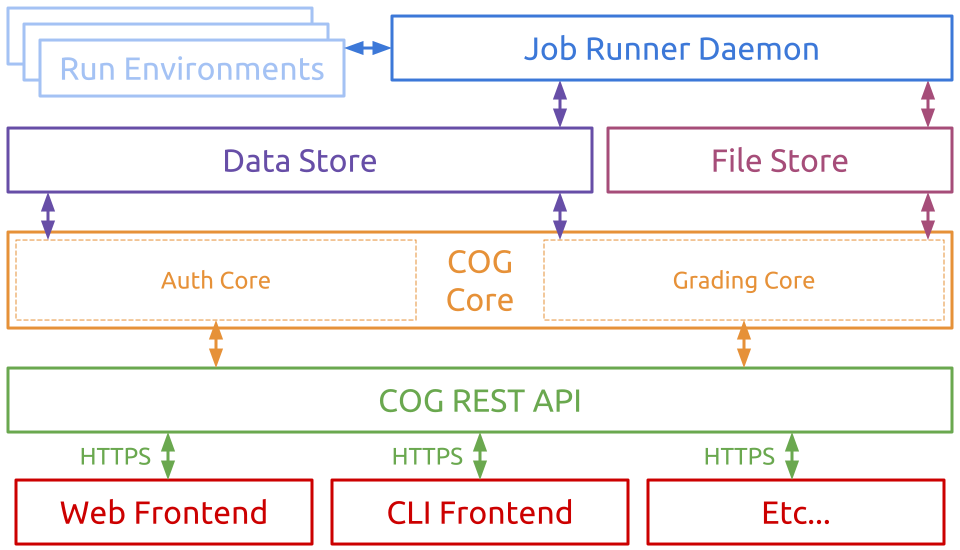
\includegraphics[width=\columnwidth]{./figs/pdf/examplefig1.pdf}
  \caption{Example Figure 1}
  \label{fig:example1}
\end{figure}

\noindent
Figure~\ref{fig:example1} is an example figure. The proceeding
sentence contains a reference to it.

\noindent
Sometimes you want thing in {\bf bold}.

\noindent
Or in {\em italics}.

\noindent
Or in \texttt{type-write font}.

\noindent
Sometime you need to do some math: $9/3=3$.

\noindent
Or ``a quote.''

\noindent
Or add a bullet list:

\begin{packed_item}
\item Item A
\item Item B
\item Item C
\end{packed_item}

\noindent
Or a numbered list:

\begin{packed_enum}
\item Item 1
\item Item 2
\item Item 3
\end{packed_enum}

\noindent
Or a definitions list:

\begin{packed_desc}
\item[Item I:] This is item 1 
\item[Item II:] This is item 2
\item[Item III:] This is item 3
\end{packed_desc}

% Note: The ``packed'' variants of the above items are my own and are
% defined in macros.tex. They are more tightly spaced versions of the
% standard LaTeX enumerate, itemize, and description environments.

\bibliographystyle{acm}
\bibliography{refs}

\end{document}
